
\section{Part I - Mathematical modelling} \label{sec:part1}
\begin{figure}[h!] 
    \begin{center}
    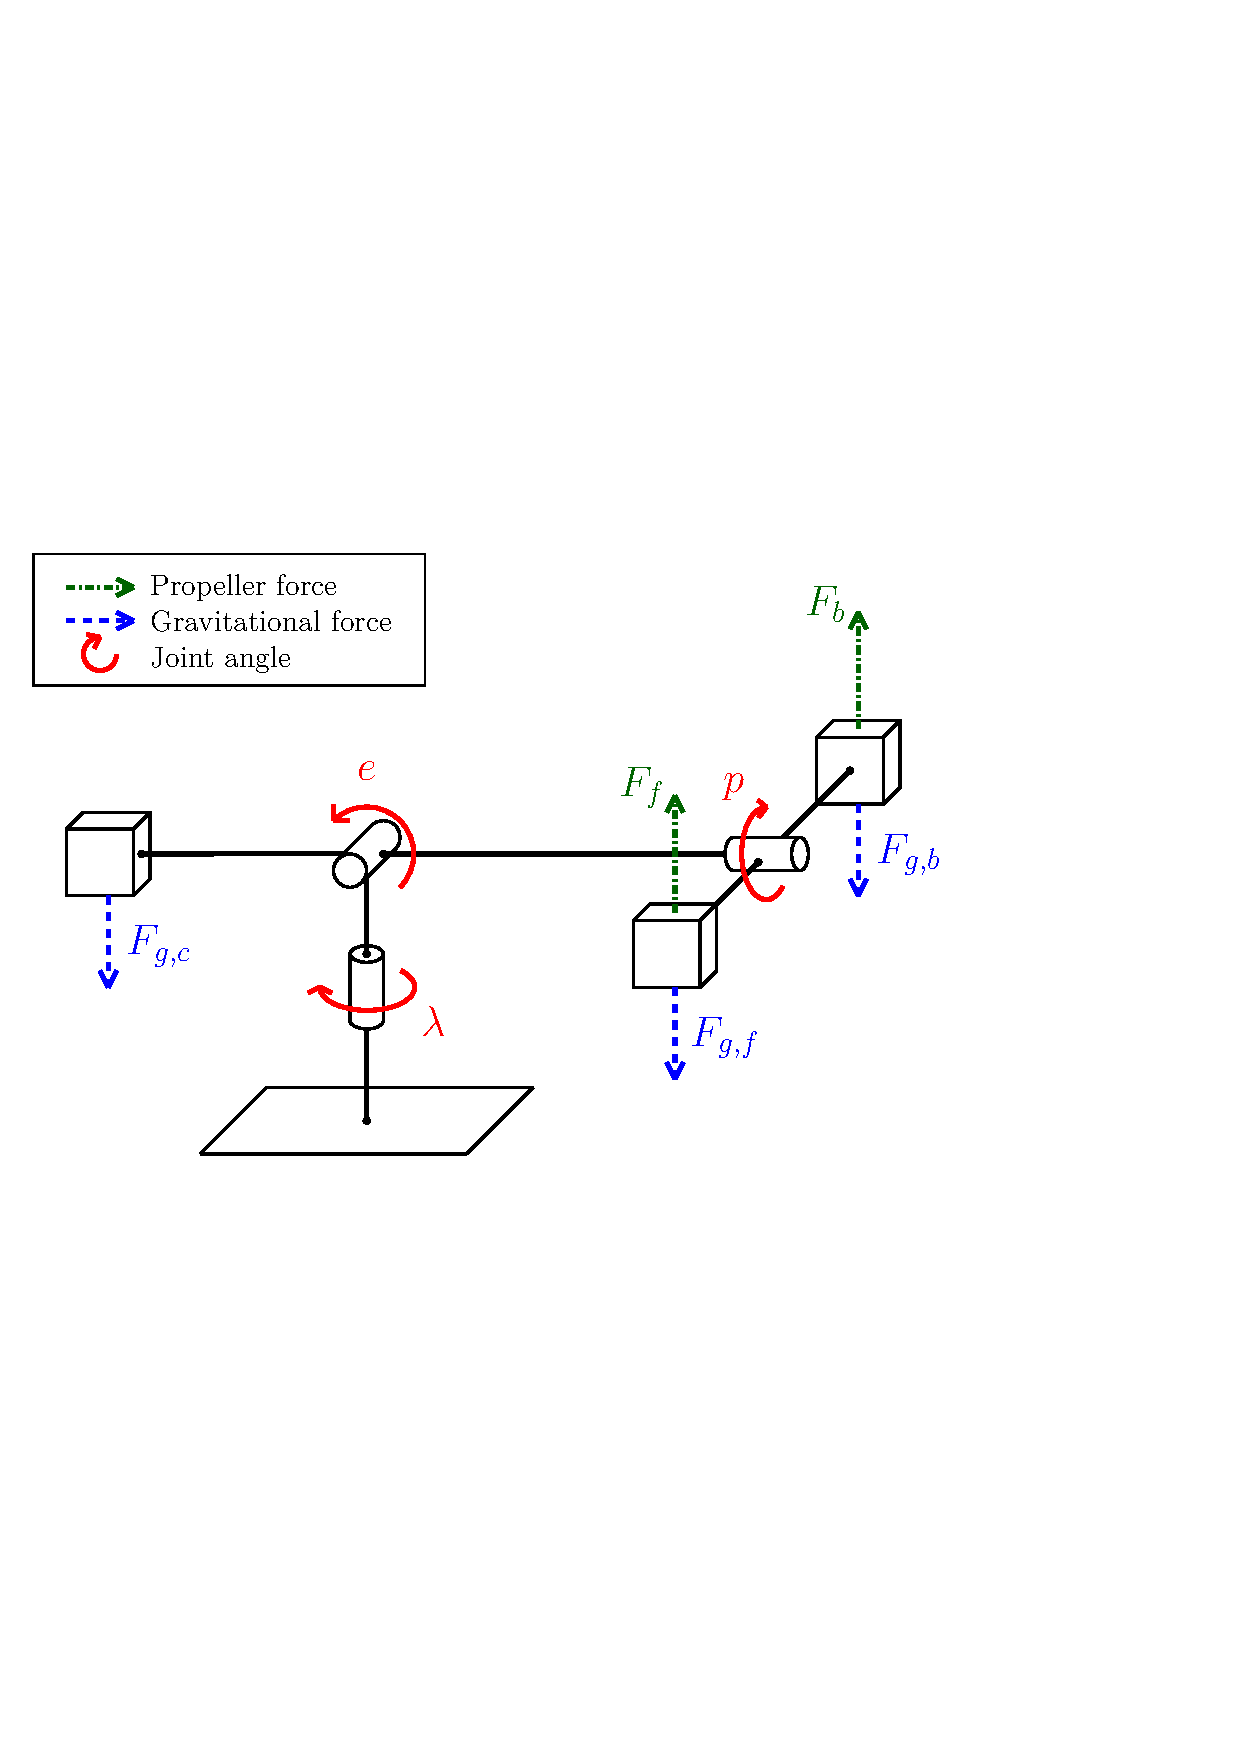
\includegraphics[scale=0.65]{Figures/forces.pdf}
    \caption{Modeling: The model is from the source file of the lab exercise. This model represents chosen positive direction of forces and rotations.} 
    \label{fig:helic_model}  
    %Smart måte å lage labels: https://en.wikibooks.org/wiki/LaTeX/Labels_and_Cross-referencing
    \end{center}
\end{figure}
\begin{figure}[h!] 
    \begin{center}
    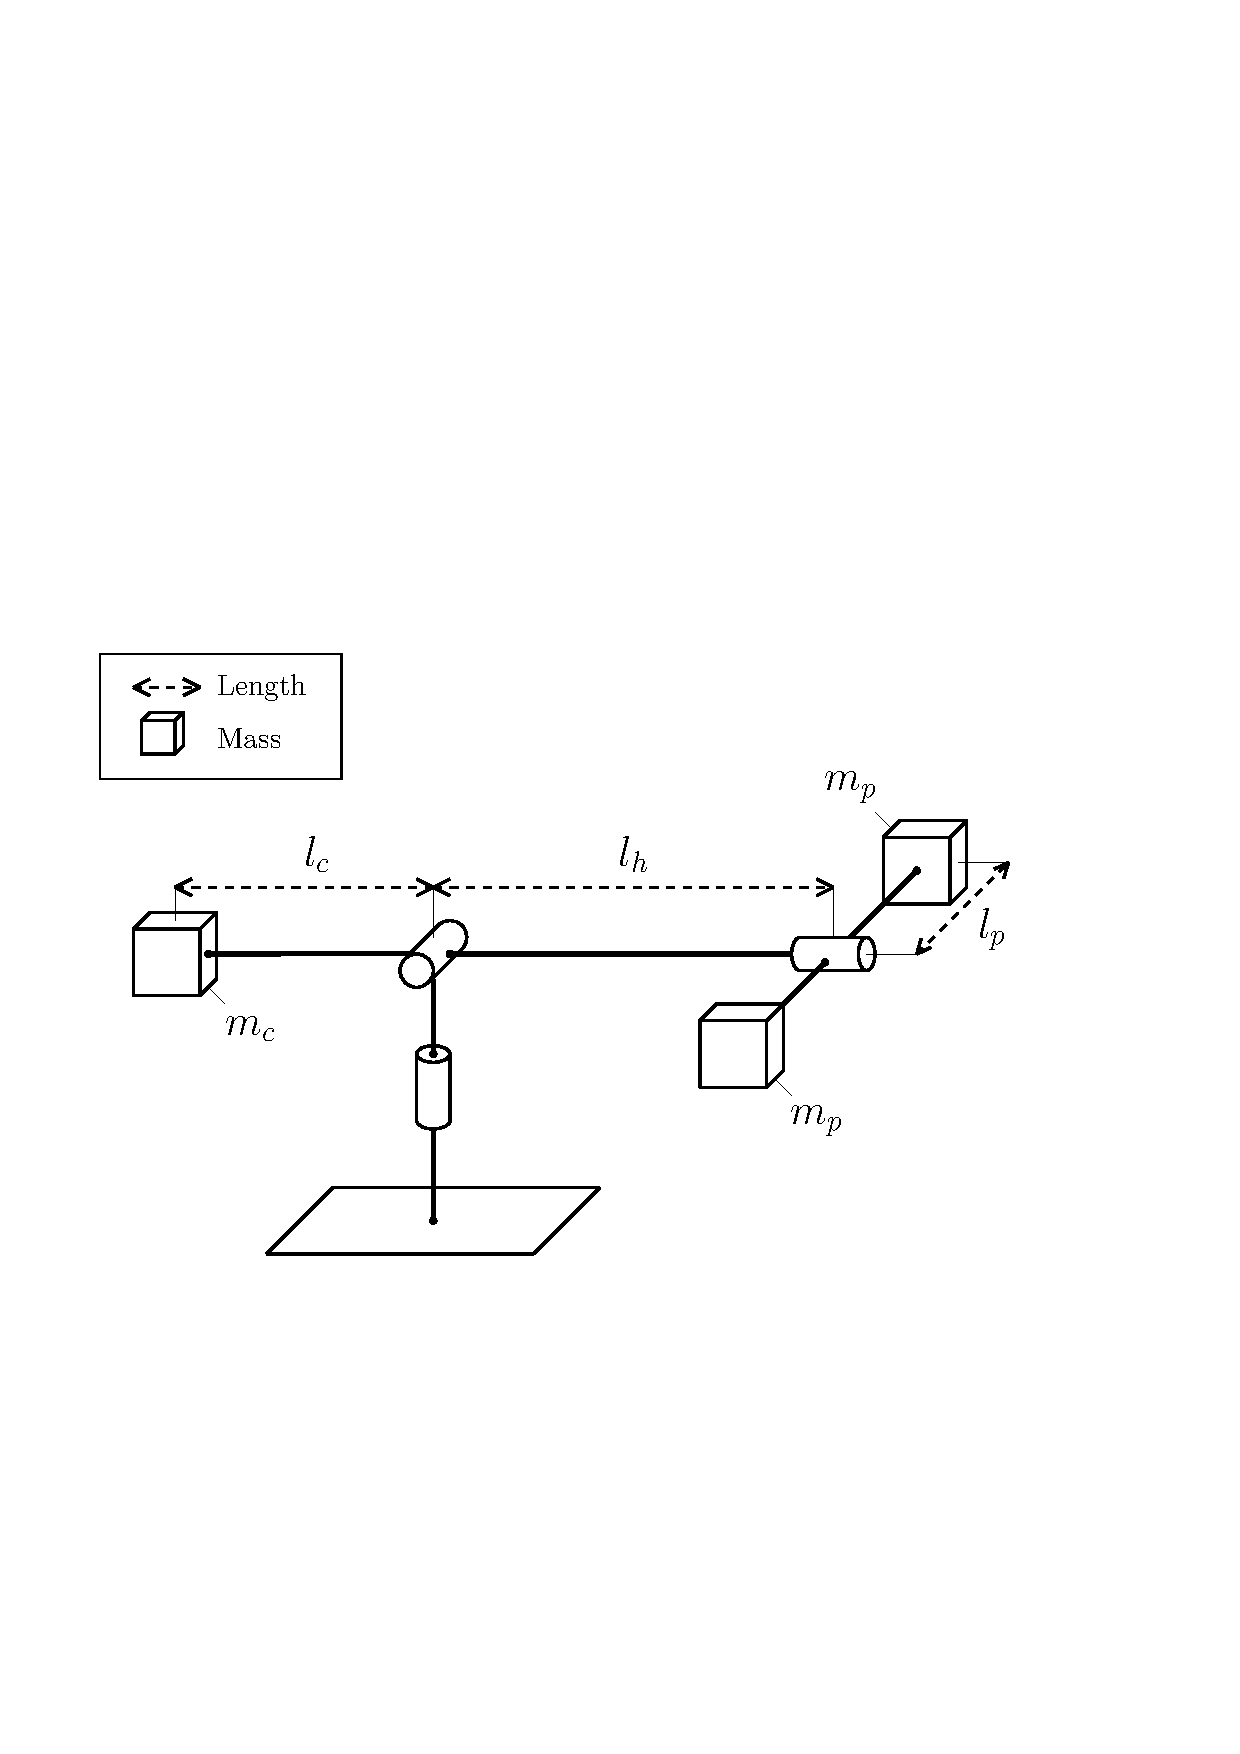
\includegraphics[scale=0.65]{Figures/masses.pdf}
    \caption{Same model with names of lengths and masses used in calculations from the source file of the exercise} 
    \label{fig:helic_model_masses}  
    %Smart måte å lage labels: https://en.wikibooks.org/wiki/LaTeX/Labels_and_Cross-referencing
    \end{center}
\end{figure}
\Cref{fig:helic_model} and \cref{fig:helic_model_masses} shows a model of the helicopter. The two motors are represented with two masses. There are three rotation points: pitch $p$, elevation angle $e$ and travel angle $\lambda$. Pitch angle is defined as zero when the helicopter head is horizontal, and elevation angle is zero when the arm of the helicopter is horizontal, this will be implemented later. 

%%% 5.1
\subsection{Problem 1}
Following equations was given from the lab problem
    \begin{equation} \label{K_f}
    F_f = K_f V_f
    \end{equation}
    \begin{equation} \label{K_b}
    F_b = K_f V_b
    \end{equation}
To find an expression for pitch-, elevation- and travel angle Newtons second law for rotation \eqref{eq:n2} was used with centre and direction as defined in \cref{fig:helic_model} and lengths and masses as shown in figure \ref{fig:helic_model_masses}.
    \begin{equation}\label{eq:n2}
     \sum \tau = I \ddot \Theta = J_p \ddot p
    \end{equation}
Using Newton's second law for the pitch equation
    \begin{equation*}\label{eg of pitc}
        J_p \ddot p = l_p  (F_f -  F_{g,f} -  F_b +   F_{g,b})
    \end{equation*}
by inserting equations \eqref{K_f} and \eqref{K_b}
    \begin{equation*}
        J_p \ddot p = l_p  (K_f V_f - m_p g - K_f V_b + m_p g)
    \end{equation*}
    \begin{equation*}
        J_p \ddot p = l_p  (K_f (V_f - V_b))
    \end{equation*}
    \begin{equation*} 
        J_p \ddot p = l_p K_f  V_d 
    \end{equation*}
a constant $L_1$ was defined as
    \begin{equation}\label{con:L_1}
        L_1 = l_p  K_f 
    \end{equation}
    %%Elevation ligning:
Using Newton's second law for the elevation equation
    \begin{equation*}\label{eq of angle}
        I \ddot \Theta = J_e \ddot e = l_c F_{g,c} + l_h [( F_f + F_b) - (F_{g,f} + F_{g,b})]
    \end{equation*}
    \begin{equation*}
        J_e \ddot e = l_c  m_c  g \cos(e) + l_h[K_f\cos(p)(V_f+ V_b) -2 m_p g\cos(e)]
    \end{equation*}
    \begin{equation*}
        J_e \ddot e = (l_c m_c - 2l_h m_pg)\cos(e) + l_h K_f V_s \cos(p)
    \end{equation*}
with two constants defined as
    \begin{equation}
        L_2 = (l_c m_c - 2l_h m_p)g 
    \end{equation}
    \begin{equation}
        L_3 = l_h  K_f 
    \end{equation}
    %% Travel ligning
Using Newton's second law for the travel angle
    \begin{equation*}\label{eg og landa}
        J_\lambda \ddot \lambda = l_\lambda (F_f + F_b) \sin (-p)
    \end{equation*}
where $l_\lambda$ is the length from the middle pole to the motors, and can be decomposed to $l_\lambda = l_h \cos(e)$
    \begin{equation*}
        J_\lambda \ddot \lambda= l_h \cos(e) K_f (V_f + V_b) \sin (-p)
    \end{equation*}
    \begin{equation*}
        J_\lambda \ddot \lambda= -K_f l_h V_s \cos(e) sin(p)
    \end{equation*}
a constant $L_4$ was defined as
    \begin{equation}
        L_4 = -l_h K_f
    \end{equation}
The final expressions for pitch-, elevation- and travel angle could now be written as
\begin{equation}
    J_p \ddot p = L_1 V_d
    \label{2a}
\end{equation}
\begin{equation}
    J_e \ddot e = L_2 \cos(e) + L_3 \cos(p)
    \label{2b}
\end{equation}
\begin{equation}
    J_{\lambda} \ddot \lambda = L_4 V_s \cos(e) \sin(p)
    \label{2c}
\end{equation}

\subsection{Problem 2}
The goal with this problem was to find a linearized model of the system around the equilibrium point $(p,e,\lambda)^T = (p^*,e^*,\lambda^*)^T$, where this point was the origin ($p^* = e^* = \lambda^* = 0$). First expressions for the voltages $V_s^* = V_s$ and $V_d^* = V_d$ had to be found such that $\dot{p} = \dot{e} = \dot{\lambda} = 0$ for $(p,e,\lambda)^T = (p^*,e^*,\lambda^*)^T$. By using equations \eqref{2a} and \eqref{2b} and that $\dot{x} = 0 \rightarrow \ddot{x} = 0$
\begin{equation*}
    \ddot{p} = \ddot{p}^*, V_d = V_d^*
\end{equation*}
\begin{equation*}
    J_p\ddot{p}^* = L_1 V_d^* = 0
\end{equation*}
\begin{equation}\label{eq:Vdstar}
    V_d^* = 0
\end{equation}

\begin{equation*}
    \ddot{e} = \ddot{e}^*, V_s = V_s^*
\end{equation*}
\begin{equation*}
    J_e \ddot{e}^* = L_2 \cos(e^*) + L_3 V_s^* \cos(p^*) = 0
\end{equation*}
\begin{equation}\label{eq:Vsstar}
    V_s^* = - \frac{L_2}{L_3}
\end{equation}
The system could now be linearized by using the coordinate transformation
\begin{equation*}
    \tilde{x} =
    \begin{bmatrix}
        \tilde{p}\\ \tilde{e}\\ \tilde{\lambda}
    \end{bmatrix}
    =
    \begin{bmatrix}
        p\\ e\\ \lambda
    \end{bmatrix}
    -
    \begin{bmatrix}
        p^*\\ e^*\\ \lambda^*
    \end{bmatrix},
    \tilde{u} =
    \begin{bmatrix}
        \tilde{V_s}\\ \tilde{V_d}
    \end{bmatrix}
    =
    \begin{bmatrix}
        V_s\\ V_d
    \end{bmatrix}
    -
    \begin{bmatrix}
        V_s^*\\ V_d^*
    \end{bmatrix}
\end{equation*}
The original $\dot{x}$ was found with equations \eqref{2a} - \eqref{2c} defined as $h_1(x,u) - h_3(x,u)$, $\tilde{\textbf{A}}$ and $\tilde{\textbf{B}}$ defined with equations for linearization. These matrices was used to get the system on the form
\begin{equation*}
\dot{\tilde{\textbf{x}}} = {\tilde{\textbf{A}} \tilde{\textbf{x}}} + {\tilde{\textbf{B}} \tilde{\textbf{u}}}.
\end{equation*}
\begin{subequations}
    \begin{align}
    \dot{\textbf{x}} &= \begin{bmatrix}\label{Lin matrix}
        h_1(x_1, x_2, u_1, u_2)\\
        h_2(x_1, x_2, u_1, u_2)\\
        h_3(x_1, x_2, u_1, u_2)
    \end{bmatrix}\\
    \tilde{\textbf{A}} &=\begin{bmatrix}{\label{A matrix}}
        \frac{\partial h_1}{\partial p} & \frac{\partial h_1}{\partial e}  & \frac{\partial h_1}{\partial \lambda}\\
        \frac{\partial h_2}{\partial p} & \frac{\partial h_2}{\partial e}  & \frac{\partial h_2}{\partial \lambda}\\
        \frac{\partial h_3}{\partial p} & \frac{\partial h_3}{\partial e}  & \frac{\partial h_3}{\partial \lambda}\\
    \end{bmatrix}\\
    \tilde{\textbf{B}} &= \begin{bmatrix}{\label{B matrix}}
        \frac{\partial h_1}{\partial \tilde{V_s}} & \frac{\partial h_1}{\partial \tilde{V_d}}\\
        \frac{\partial h_2}{\partial \tilde{V_s}} & \frac{\partial h_2}{\partial \tilde{V_d}}\\
        \frac{\partial h_3}{\partial \tilde{V_s}} & \frac{\partial h_3}{\partial \tilde{V_d}}\\
    \end{bmatrix}
    \end{align}
\end{subequations}
After some calculation the $\tilde{\textbf{A}}$ and $\tilde{\textbf{B}}$ matrix was found to be 
    \begin{align}
    \tilde{\textbf{A}} &=\begin{bmatrix}
        0 & 0  & 0\\
        -\frac{L_3 V_s}{J_e} \sin(p) & -\frac{L_2}{J_e}\sin(e)  & 0\\
        \frac{L_4 V_s}{J_\lambda}\cos(e) \cos(p) & -\frac{L_4}{J_\lambda} \sin(e) \sin(p)  & 0\\
    \end{bmatrix}
    \end{align}
        \begin{align}
    \tilde{\textbf{B}} &= \begin{bmatrix}
        0 & \frac{L_1}{J_p}\\
        \frac{L_3}{J_e} \cos(p) & 0\\
        \frac{ L_4}{J_ \lambda} \cos(e) \sin(p) & 0\\
    \end{bmatrix}
    \end{align}
Then by inserting the point of equilibrium presentet earlier
    \begin{align}
    \tilde{\textbf{A}} &=\begin{bmatrix}{\label{A matrix sol}}
        0 & 0  & 0\\
        0 & 0  & 0\\
        \frac{L_4 V_s^*}{L_\lambda} & 0  & 0\\ %Men blir det det V_s* eller V_s??? 
    \end{bmatrix}
    \end{align}

    \begin{align}
    \tilde{\textbf{B}} &= \begin{bmatrix}{\label{B matrix sol}}
        0 & \frac{L_1}{J_p}\\
        \frac{L_3}{J_e} & 0\\
        0 & 0\\
    \end{bmatrix}
    \end{align}
The system $\dot{\tilde{\textbf{x}}} = {\tilde{\textbf{A}} \tilde{\textbf{x}}} + {\tilde{\textbf{B}} \tilde{\textbf{u}}}$ can be written as
\[
\begin{bmatrix}
    \ddot{\tilde p} \\
    \ddot{\tilde e}\\
    \ddot{\tilde \lambda}
\end{bmatrix}
=
\begin{bmatrix}
    0 & 0  & 0\\
    0 & 0  & 0\\
    \frac{L_4 V_s^*}{L_\lambda} & 0  & 0\\ %Men blir det det V_s* eller V_s??? 
\end{bmatrix}
\begin{bmatrix}
    \tilde {p} \\
    \tilde{e}\\
    \tilde{\lambda}\\
 \end{bmatrix}
 + 
 \begin{bmatrix}
     0 & \frac{L_1}{J_p}\\
    \frac{L_3}{J_e} & 0\\
    0 & 0\\
\end{bmatrix}
\begin{bmatrix}
    \tilde{V_s}\\
    \tilde{V_d}\\ 
\end{bmatrix}
\]
Now $\ddot{\tilde{p}}$, $\ddot{\tilde{e}}$ and $\ddot{\tilde{\lambda}}$ can easily be found
\begin{subequations}
    \begin{gather}
        \ddot{\tilde{p}} =  K_1 \tilde{V_d}\label{6a}\\
        \ddot{\tilde{e}} = K_2 \tilde{V}_s\label{6b}\\
        \ddot{\tilde{\lambda}} = K_3 \tilde{p} \label{6c}
    \end{gather}
\end{subequations}

\begin{subequations}
	\begin{gather}
		K_1 = \frac{L_1}{J_p} = \frac{K_f}{2 m_p l_p}\label{eq:K_1}\\
		K_2 = \frac{L_3}{J_e} = \frac{l_h K_f}{m_c l_{c}^2 + 2m_p l_{h}^2}\label{eq:K_2}\\
        K_3 =\frac{L_4 V_s^*}{J_{\lambda}} = g \frac{m_c l_c - 2 m_p l_h}{m_cl_{c}^2 + 2m_p(l_{h}^2+l_{p}^2)} \label{eq:K_3}
	\end{gather}
\end{subequations}


\subsection{Problem 3}
Now comes the first attempt to control the helicopter. This was done by connecting the x- and y-axis directly to the voltages $V_d$ and $V_s$ (see Appendix B for implementation in Simulink). Gains were added to both voltages to make the helicopter easier to control, and these were treated as inputs to the voltages. Since the motors did not need a large voltage difference, a gain on 0.8 was added to the $V_d$ input. A gain on 10 to $V_d$ was guessed to be the input needed to get the helicopter running, but it was very hard to control. After trying out different gains the helicopter was still very difficult to control, and the physical behavior did not correspond well to the theoretical model in equation \eqref{2a} - \eqref{2c}. 
\newline\newline
There is a couple of reasons why these two does not correlate, and the main reason is because of the simplification of the system. The equations \eqref{2a} - \eqref{2c} does not take drag or other losses of energy into consideration. The theoretical system \eqref{6a} - \eqref{6c} is linearized and therefore will not correctly map an nonlinear system as a helicopter. Only masses from counter weight and motors are used in calculations and the helicopter has physical limitations for angles and input voltage to the motors. All these factors simplifies the model and these discrepancies makes the theoretical model differs from the physical behavior.

\subsection{Problem 4}
The equilibrium state was now redefined such that elevation is zero when the arm between the helicopter head and the elevation axis is horizontal. By scoping the elevation in Simulink, horizontal arm was when the helicopter was 30 degrees from the table, and an offset of 30 was subtracted from the elevation. The pitch was scoped and found to be zero while the helicopter head was resting on the table (there were a few exceptions of the pitch, but this was due to imperfections of the table surface). These scopes are shown in figure \ref{fig:offsets}. A simple $\frac{\pi}{180}$ gain was used to convert the encoder outputs from degrees to radians.
\newline\newline
To use the linearized equations of motion \eqref{6a} - \eqref{6c}, the motor force constant $K_f$ had to be determined. This was done by observation of $V_s$ by scopes while the helicopter was in the new point of equilibrium for elevation. $V_s$ was found to be $V_s = 6.75V$. To calculate $K_f$, equation \eqref{2b} was used with $\ddot{e} = 0$ and the point of equilibrium $e = e^* = p = p^* = 0$.

\begin{equation*}
    -L_2 = L_3 V_s, L_3 = K_f l_h
\end{equation*}
\begin{equation}\label{eq:K_f}
    K_f = - \frac{L_2}{l_h V_s} = 0.1480
\end{equation}
The Simulink system was made such that $V_s^*$ was added to $\tilde{V_s}$ (see figure \ref{fig:vs_add}), the helicopter could now reach the point of equilibrium on it's own.

\begin{figure}[H]
\begin{subfigure}{0.5\textwidth}
    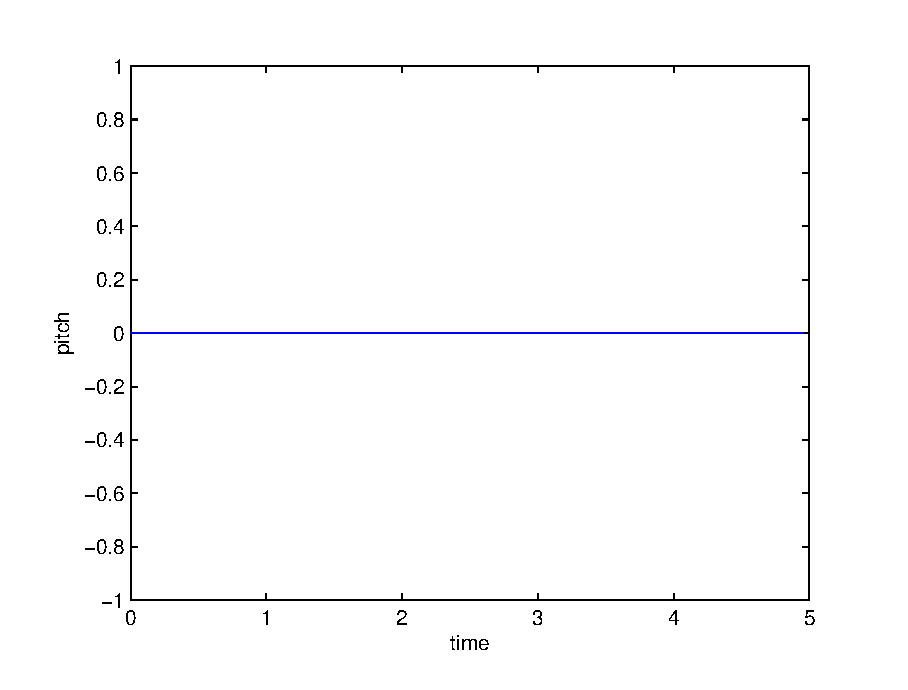
\includegraphics[width=1\linewidth]{Part1_Pictures/pitch_offset.eps} 
\end{subfigure}
\begin{subfigure}{0.5\textwidth}
    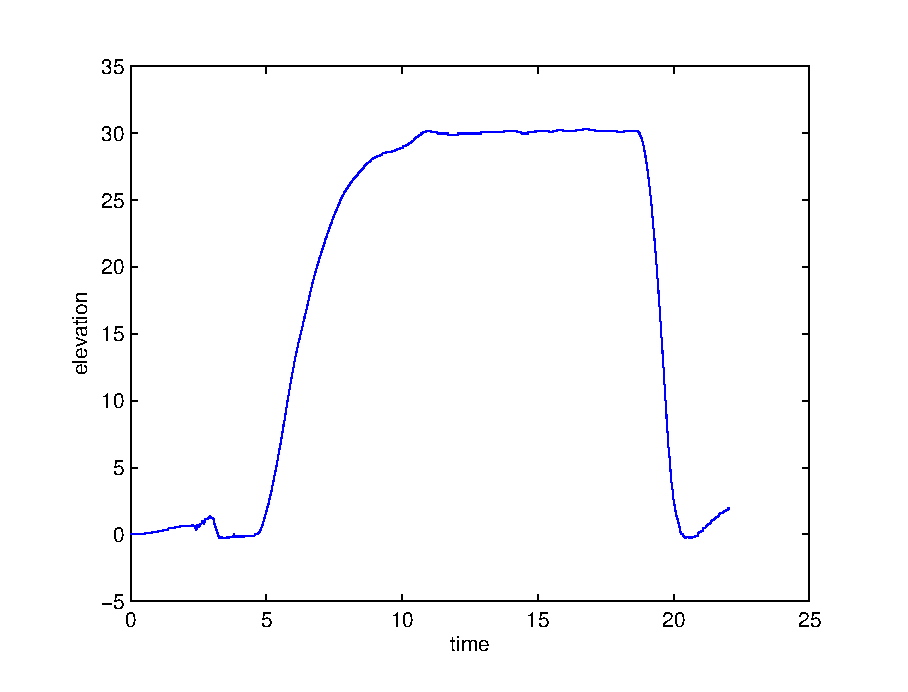
\includegraphics[width=1\linewidth]{Part1_Pictures/elevation_offset.eps}
\end{subfigure}
\caption{Offset values for the helicopter in the given point of equilibrium}
\label{fig:offsets}
\end{figure}